\section{Aufbau und Durchführung}
\label{sec:Durchführung}

\subsection{Aufbau}
In \autoref{fig:Aufbau} ist der Versuchsaufbau zu finden.
Als Gamma-Strahlungsquelle wird $\ce{^{137}Cs}$ verwendet.
Eine Bleiabschirmung mit einem Loch mit $\SI{3}{\milli\metre}$ Durchmesser dient zur Kollimierung.
Daneben befindet sich die verstellbare Plattform für den Würfel.
Dadurch kann der Würfel um seine eigene Achse gedreht, sowie an der y-Achse verschoben werden.
Zum Schluss ist der Szintillationsdetektor, der die abgeschwächten Strahlungen misst.

Das Material des Szintillationsdetektor bzw. die Atome werden durch die Gamma-Strahlung angeregt.
Durch Emission eines Photons kehrt das angeregte Atom zurück zum Grundzustand.
Das verwendete Material des Szintillationsdetektors ist ein NatriumIodidkristall.
Am Szintillationsdetektor sind Photomultiplier, Diskriminator und Multichannelanalyzer angeschlossen.
Das eben emittierte Photon trifft auf die Photokathode im Photomultiplier auf und löst aufgrund des Photoeffekts ein Elektron aus.
Durch eine angelegte Spannung kann der Strom gemessen werden.
Der Diskriminator sorgt für eine Rauschminderung und der Multichannelanalyzer nimmt die gemessenen  Werte auf und zeigt sie in einem Histogramm an.

Bei den zu untersuchenden Objekten handelt es sich um 3x3x3cm Würfel bestehend aus einem Aluminiumgehäuse, welches die inneren 27 Elementarwürfel zusammenhält.
Insegesamt werden vier Würfel durchstrahlt.
Würfel 1 ist ein hohler Würfel bzw. besteht nur aus dem Gehäuse.
Würfel 2 und 3 sind mit Elematarwürfeln gefüllt und sind jeweils homogen.
Würfel 4 besteht aus einer heterogenen Mischung aus den Elementarwürfeln von Würfel 2 und 3.


\begin{figure}[H]
    \centering
    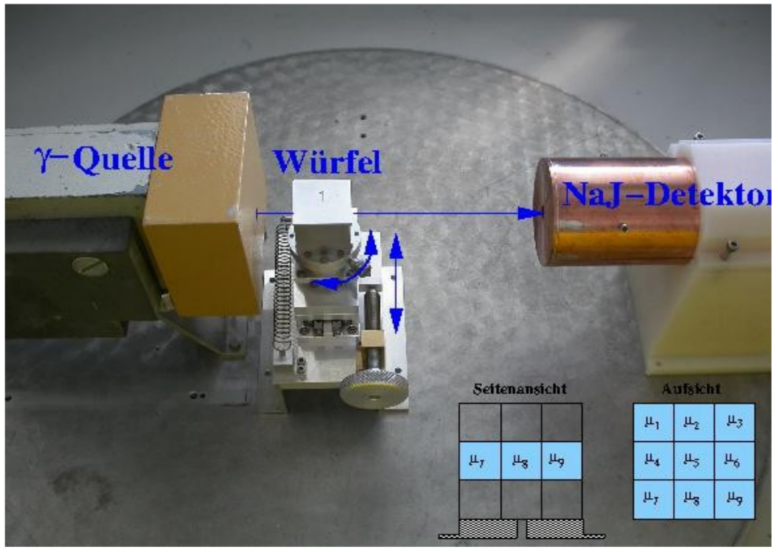
\includegraphics[width=\textwidth]{bilder/Aufbau.png}
    \caption{Der Versuchsaufbau. Links befindet sich die Gamma-Quelle, mittig die verstellbare Plattform für die Würfel und rechts ist der Szintillationsdetektor zu sehen. \cite{anleitung}}
    \label{fig:Aufbau}
\end{figure}

\subsection{Durchführung}
Zunächst wird das Spektrum der $\ce{^{137}Cs}$ Quelle aufgenommen.
Dafür wird für $\SI{300}{\second}$ lang gemessen, ein Würfel wird hier noch nicht eingesetzt.
Danach werden die insgesamt vier Würfel durchstahlt und die Messwerte aufgenommen.
Es wird das a priori Wissen genutzt, dass Würfel 1, 2 und 3 homogen sind.
Somit werden für die homogenen Würfel nur 3 bzw. 6 Projektionsmessungen statt 12 durchgeführt.
Bei Würfel 4 werden alle 12 Projektionen vermessen.
Die Messzeit für eine Strahlrichtung beträgt für jeden Würfel $\SI{300}{\second}$.